\documentclass[a4paper]{article}

\usepackage[english]{babel}
\usepackage[utf8]{inputenc}
\usepackage{amsmath}
\usepackage{hyperref}
\usepackage{subcaption}
\usepackage{graphicx}
\usepackage[colorinlistoftodos]{todonotes}

\title{Q4. Monte Carlo: (Dr. Shanbhag )\\Summer 2016}


\author{Amirhessam Tahmassebi}

\date{\today}

\begin{document}
\maketitle


 

\section*{Method}


For Ellipse $E_1$ we have: \\

$$E_1 : \frac{x^2}{a^2} + \frac{y^2}{b^2} = 1$$
We know that Ellipse $E_2$ has the same shape as $E_1$ but it is rotated counter clockwise for $\frac{\pi}{3}$, then we have: \\
$$\begin{bmatrix}
    x_{new}  \\
    y_{new}  \\
   
\end{bmatrix}
 = \begin{bmatrix}
    cos\theta & -sin\theta  \\
    sin\theta & cos\theta  \\
   
\end{bmatrix} 
\begin{bmatrix}
    x \\
    y\\
   
\end{bmatrix}
= \begin{bmatrix}
    xcos\theta + ysin\theta \\
    xsin\theta - ycos\theta \\
   
\end{bmatrix}
$$
Also, we know that the center of $E_2$ , $O'$ is not $ O (0,0)$, but we know $OO' =\delta = 0.1 $. Using the right-angle triangle we have with legs of $x_{new}$ and $y_{new}$ which leads us to: 
$$O' =(x_{new},y_{new}) = (\delta cos(\frac{\pi}{3}) , \delta sin(\frac{\pi}{3}))$$
$$E_2 :  \frac{[(x-x_{new})cos\theta + (y-y_{new})sin\theta]^2}{a^2} +
\frac{[(x-x_{new})sin\theta - (y-y_{new})cos\theta]^2}{b^2} = 1$$
For all the equations, $ a = 2 $ and $ b =1$. \\
With using simple monte carlo with considering the criteria that each point should be true for:  $E1 <= 1$ AND $E2 <=1$
For The Area we will have:
$$Area = 3.8682 $$

\begin{figure}[ht]
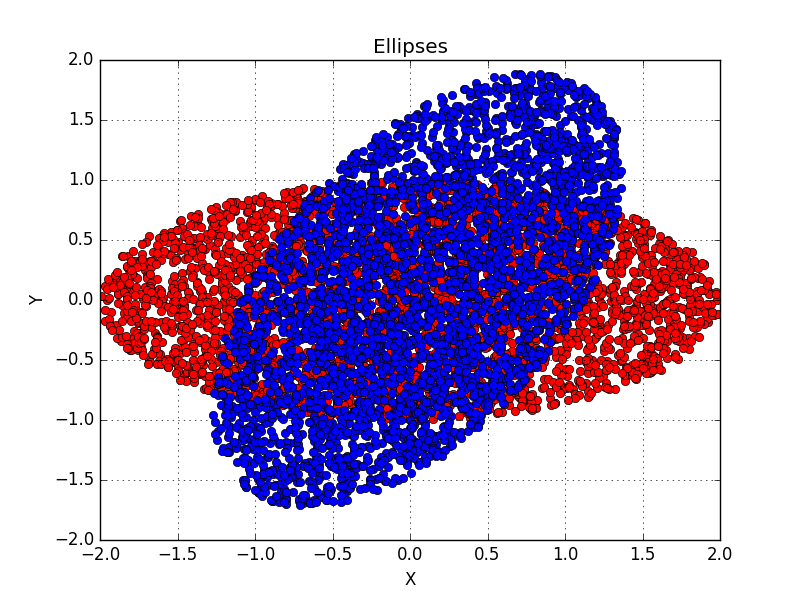
\includegraphics[scale=.65]{01.png}
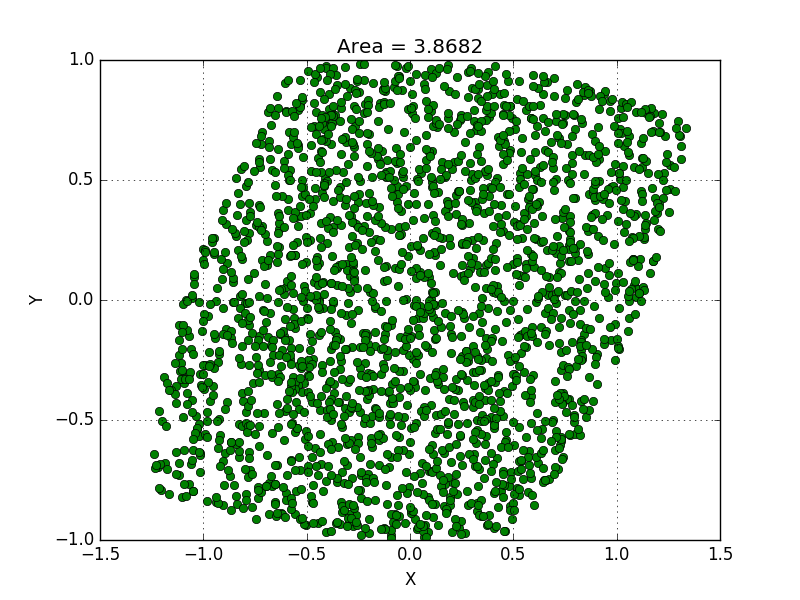
\includegraphics[scale=.65]{02.png}
\end{figure}









\end{document}